\chapter{Software Defined Networking} \label{chap:sdn} %% chapter 3

Computer networking is a vital part of the services that are offered today, and as such, the performance in technology backing these services is central to the quality of these services. As the service providers reorganize their
data centers in the cloud computing domain, enabling several improvements in the predictability, quality of service and ease of use of their services. New technologies are then required to make sure that their services are adapted
to the fast changing landscape of networking services. One of the most notable innovations in this field is called Software Defined Networking, because its architecture allows for two essential features

\begin {itemize}
    \item \textbf{Separation of network planes} SDN allows for the separation of the network control plane from the data forwarding plane by having network "intelligence" present in the network controllers, and having them
control the forwarding elements that live in the Data Plane
    \item \textbf{Centralization of network management functions} By isolating the management on a separate plane, there is possibility of developing a single controller that can regulate the entire network, having unrestricted access to every element present in the network, simplifying management, monitoring, application of QoS policies, flow optimization, ...
\end {itemize}

In this chapter we explore the essential characteristics of SDN, the technologies that provide the back end for the development of this technology, and current implementations of the most popular SDN controllers, so that we can 
see the features that should be present while developing a management interface for SDN controllers.

\section {OpenStack}
\section {OpenFlow}

As the growth of the networking infrastructure of the past few decades became evident, the need for an enviroment that allows for experimentation and testing of different protocols and equipment became evident. If networking 
research would depend on the previously existing methods, then new ways of creating and developing protocols would become increasingly hard to implement and develop. As such, there was need for a framework that could 
enable testing of new ideas on close to realistic settings. So, on 28 February 2011 the version 1.1 of OpenFlow was released, and this proposal quickly became the standard for networking in a Software Defined Network. Since
2011, this protocol has suffered some revisions, and the latest version supported is version 1.5.1. Since this framework has evolved quite a bit, this section focuses on the versions 1.3, which are the versions that 
are used in development of this dissertation. 
\par Several reasons led to the quick standardization of this protocol, which are related not only to the initial requirements of the platform, like the capability of supporting high-performance and low-cost implementations, 
and the capability of ensuring separation between production and testing traffic, but also the extensibility that the open source development model provides, removing the limitations that closed or commercial solutions give the 
network researchers.
\par The big advantage of OpenFlow is that it is, from the data forwarding plane point of view, easy to process. Since the control decisions are made by the controller, which lives in a separate plane, all the switch needs to do
is correctly match the incoming packets, and forward them according to the rules established by the controller. The components that are part of this system and enable this functionality are:

\begin {itemize}
    \item \textbf {FlowTables} This element describes the main component of the switching capabilities of the OpenFlow switch. Inside the switch there are several flow tables that can be used to match incoming packets,
and process them in the rules that are specified by the controller. These rules can contain actions that affect the path of the packets, and these actions usually include forwarding to a port, packet modification, among
others. Classification is done via matching one or more field present in the packet, for example the switch input port, the MAC and IP addresses, IP protocol, basically all information required to correctly process the 
incoming packet. The required actions for an OpenFlow switch are the capability of forwarding to a set of output ports, allowing the packet to move across the network; to send them to the controller, in the case of a
miss of match; and finally the ability to drop packets, which is useful for DDoS mitigation, or more security concerns.
    \item \textbf {OpenFlow Protocol} Through the establishment of the OpenFlow Protocol between the switch and the controller, there is the definintion of several messages that allow for the control of the switch. This protocol
enables capabilities such as adding, deleting and updating flow mods in the switch, that are refered to as \textit {Controller-to-Switch} messages. Other relevant message types are the \textit {Asynchronous}, that enable the
notification of some event that ocurred, this type includes the Packet-In message, that is a type of message that is sent to the controller when a certain packet has no match in the flow tables present in the switch; and the 
\textit{ Synchronous} message that enable functionality such as the Hello message, that is used to start the connection between the switch and the controller.
    \item \textbf {Secure Channel} OpenFlow defines the channel that is between the switch and the controller as a secure communications channel. As the messages that are sent to the switch are critical for the correct operation 
of the system, as indicated in the previous point, the channel should be criptographically secure, to prevent spoofing of this information. As such, the channel is tipically transported over TLS.
\end {itemize}

% XXX SOURCE This images were taken from : open flow switch specification  https://3vf60mmveq1g8vzn48q2o71a-wpengine.netdna-ssl.com/wp-content/uploads/2014/10/openflow-switch-v1.3.5.pdf
\begin{figure} [h]
    \begin{subfigure}
    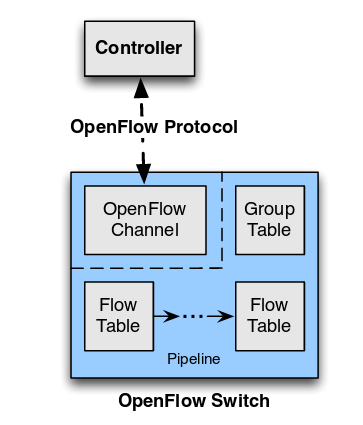
\includegraphics[width=0.25\textwidth]{sdn/open_flow_switch_pipeline}
    \end{subfigure}
    \begin{subfigure}
    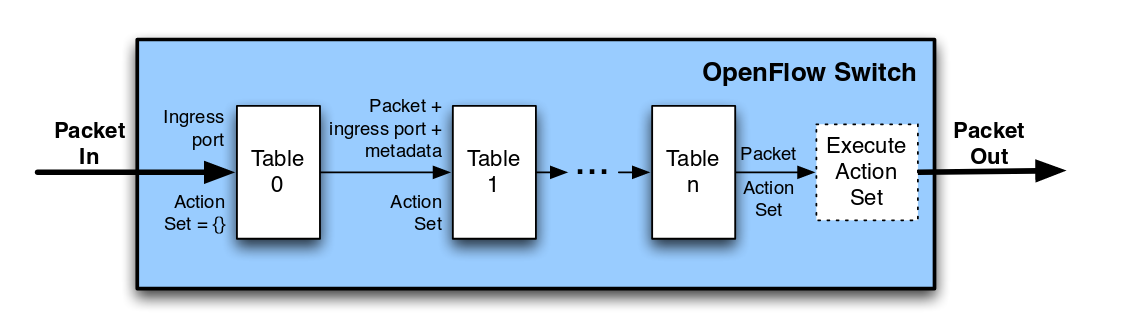
\includegraphics[width=0.6\textwidth]{sdn/open_flow_tables}
    \end{subfigure}
\caption{Images describing OpenFlow components. On the left, an overview to the entire system, and on the right a view at the table structure of the OpenFlow Switch}
\end{figure}

\subsection {Open vSwitch}

\par Although the OpenFlow protocol itself is well developed and well documented, there still needs to be support from switch applications to support this protocol. Although hardware switches are usually very expensive, and 

\subsubsection {Open vSwitch}


\section {SDN Controllers}
\subsection {Floodlight}
\subsection {OpenDaylight}
\section {SDN Northbound}
